\PassOptionsToPackage{unicode=true}{hyperref} % options for packages loaded elsewhere
\PassOptionsToPackage{hyphens}{url}
\PassOptionsToPackage{dvipsnames,svgnames*,x11names*}{xcolor}
%
\documentclass[12pt,]{article}
\usepackage{lmodern}
\usepackage{amssymb,amsmath}
\usepackage{ifxetex,ifluatex}
\usepackage{fixltx2e} % provides \textsubscript
\ifnum 0\ifxetex 1\fi\ifluatex 1\fi=0 % if pdftex
  \usepackage[T1]{fontenc}
  \usepackage[utf8]{inputenc}
  \usepackage{textcomp} % provides euro and other symbols
\else % if luatex or xelatex
  \usepackage{unicode-math}
  \defaultfontfeatures{Ligatures=TeX,Scale=MatchLowercase}
\fi
% use upquote if available, for straight quotes in verbatim environments
\IfFileExists{upquote.sty}{\usepackage{upquote}}{}
% use microtype if available
\IfFileExists{microtype.sty}{%
\usepackage[]{microtype}
\UseMicrotypeSet[protrusion]{basicmath} % disable protrusion for tt fonts
}{}
\IfFileExists{parskip.sty}{%
\usepackage{parskip}
}{% else
\setlength{\parindent}{0pt}
\setlength{\parskip}{6pt plus 2pt minus 1pt}
}
\usepackage{xcolor}
\usepackage{hyperref}
\hypersetup{
            pdftitle={Assignment FSE},
            pdfauthor={Dorian Quelle \& Frederic Denker},
            colorlinks=true,
            linkcolor=Maroon,
            filecolor=Maroon,
            citecolor=Blue,
            urlcolor=blue,
            breaklinks=true}
\urlstyle{same}  % don't use monospace font for urls
\usepackage[margin=3cm]{geometry}
\usepackage{graphicx,grffile}
\makeatletter
\def\maxwidth{\ifdim\Gin@nat@width>\linewidth\linewidth\else\Gin@nat@width\fi}
\def\maxheight{\ifdim\Gin@nat@height>\textheight\textheight\else\Gin@nat@height\fi}
\makeatother
% Scale images if necessary, so that they will not overflow the page
% margins by default, and it is still possible to overwrite the defaults
% using explicit options in \includegraphics[width, height, ...]{}
\setkeys{Gin}{width=\maxwidth,height=\maxheight,keepaspectratio}
\setlength{\emergencystretch}{3em}  % prevent overfull lines
\providecommand{\tightlist}{%
  \setlength{\itemsep}{0pt}\setlength{\parskip}{0pt}}
\setcounter{secnumdepth}{0}
% Redefines (sub)paragraphs to behave more like sections
\ifx\paragraph\undefined\else
\let\oldparagraph\paragraph
\renewcommand{\paragraph}[1]{\oldparagraph{#1}\mbox{}}
\fi
\ifx\subparagraph\undefined\else
\let\oldsubparagraph\subparagraph
\renewcommand{\subparagraph}[1]{\oldsubparagraph{#1}\mbox{}}
\fi

% set default figure placement to htbp
\makeatletter
\def\fps@figure{htbp}
\makeatother

\usepackage{dcolumn}
\usepackage{setspace}
\doublespacing
\usepackage[utf8]{inputenc}
\usepackage{float}
\usepackage{xcolor}
\usepackage{lipsum}

\title{Assignment FSE}
\author{Dorian Quelle \& Frederic Denker}
\date{Juli 19, 2020}

\begin{document}
\maketitle

\hypertarget{research-summary}{%
\subsection{Research Summary:}\label{research-summary}}

\hypertarget{keywords}{%
\subsection{Keywords}\label{keywords}}

Factorial survey experiment, donation, nudging

\newpage

\hypertarget{introduction}{%
\subsection{Introduction}\label{introduction}}

What, why and how?

\hypertarget{theory}{%
\subsection{Theory:}\label{theory}}

Relevant Theories, Hypnosis building

\hypertarget{method}{%
\subsection{Method}\label{method}}

Why FSE?

The next part will give short description of the survey methodology
itsself:

The initial planning was to run this experiment as Pen-and-Paper
Personal Interviews (PAPI). Due to the Covid-19 Pandemic this was not
feasible anymore. Therefore, we resorted to sending the PDF of the
questionnaires to the respondents and asking them to print it and send
it back.

When creating the questionnaires a sampling strategy needs to be
employed. However, our survey only has 5 dimensions with 3,3,3,2,2
levels. This means that we have a universe of 108 unique vignettes.
Including 12 vignettes for each survey we able to survey the complete
universe of vignettes in 9 surveys. We surveyed 17 individuals and each
deck at least once which should increases the validity.

\hypertarget{operationalization}{%
\subsection{Operationalization}\label{operationalization}}

For each of the twelve vignettes we presented the respondent with five
dimensions for which he or she had to respond to the question \emph{How
likely is it that you are going to donate the amount?} The following
dimensions were:

\begin{itemize}
\tightlist
\item
  The working situation of the person who will be asked to donate. The
  available options are a minimum wage job and a well paying job.
\item
  The amount of money you receive. It can be either 10, 100 or 1000
  Euros.
\item
  The origin of the money. The available options were tax refund, gift
  from mother or a bonus from work.
\item
  The channel of the money. This differentiates between whether you have
  yet to receive the money and can decide to redirect it to the cause or
  whether you have already received the money.
\item
  Lastly, the goal of the donation which can be building state capacity
  in Uganda, supporting small businesses and entrepreneurs in Uganda or
  provide education for young mothers in Uganda.
\end{itemize}

The respondent is then asked about their likelihood of donating using a
Likert Scale with 5 values. The extremes (-2 and 2) were labeled ``Very
unlikely'' and ``Very likely'' respectively.

Below you will find one example vignette as it was presented to the
respondents:

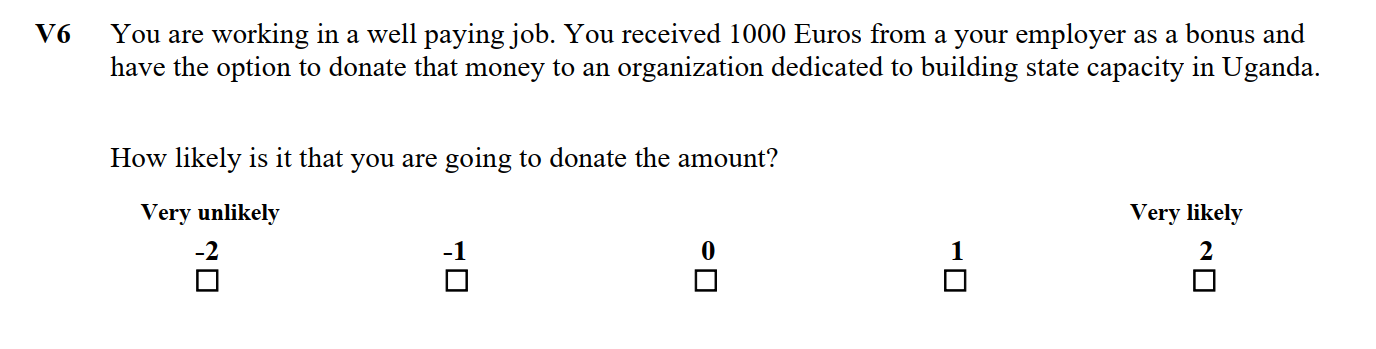
\includegraphics[width=1.05\linewidth]{Screenshot_vignette}

In addition to these 12 vignettes we asked the respondents to answer 5
questions on themselves, more specifically gender, year of birth,
country of residence and highest educational qualification.

\hypertarget{results}{%
\subsection{Results}\label{results}}

Before looking at inferential statistics it is essential to get an
overview over the data, starting with the properties of the respondents
themsselves:

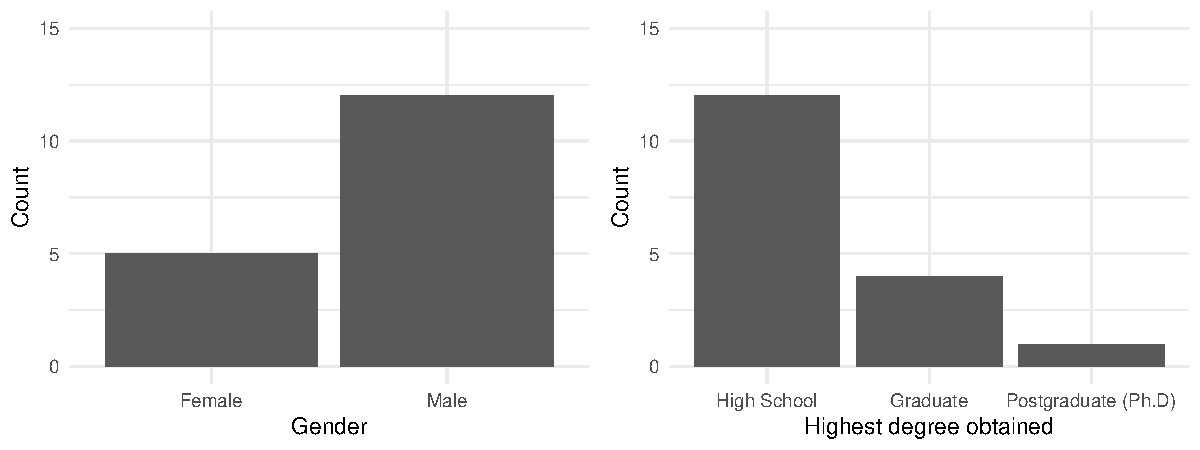
\includegraphics[width=1.05\linewidth]{FSE_paper_files/figure-latex/unnamed-chunk-2-1}

In order to give a short display of the data, the distribution of the
main outcome variable is plotted below:

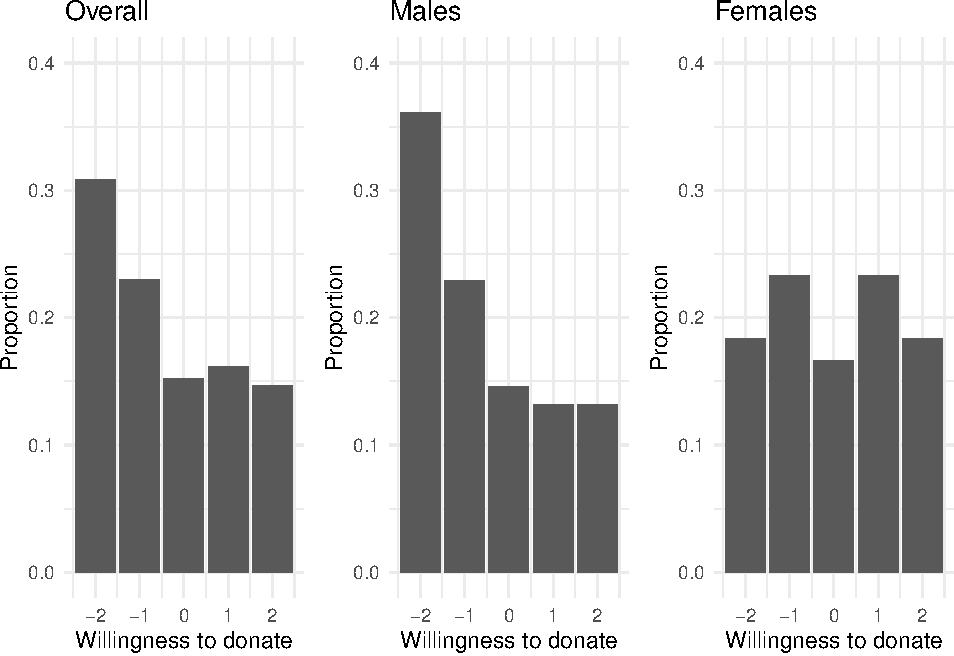
\includegraphics{FSE_paper_files/figure-latex/plotting_proportions-1.pdf}

\hypertarget{discussion}{%
\subsection{Discussion}\label{discussion}}

\end{document}
